\chapter{Caracterización y puesta en servicio}

En este capítulo se expondrán los procesos de caracterización y puesta en servicio del telescopio CPT. Para abordar los puntos de caracterización y primera luz de los objetivos propuestos para este trabajo. Se detallarán los aspectos considerados para cada una de las mediciones y los fundamentos correspondientes.

\section{Enfoque del alimentador}

Se realizaron 2 mediciones de enfoque del alimentador, una a 70 metros y otra a 186 metros. Para la primera medición se utilizó un generador de señales genérico con una LPDA de bajo ancho de banda. Luego para el resto de las mediciones se utilizó la estrella artificial de la copa de agua de la sección XX.\\

\subsection{Alimentador sin soportes a 70 metros}

En un principio el alimentador del telescopio consistía en una antena LPDA (Log Periodic Dipole Array) de 296 MHz a 6 GHz, de ultra ancho de banda, con una ganancia de aproximadamente 9 dBi. Con el receptor instalado en esta antena, se procedió a realizar el enfoque del alimentador. Para esta etapa se retiró el soporte tetrápodo y se instaló el alimentador en un trípode auxiliar sostenido por un tubo de PVC para lograr la altura del centro del reflector de 2 metros.\\

\begin{figure}
    \centering
    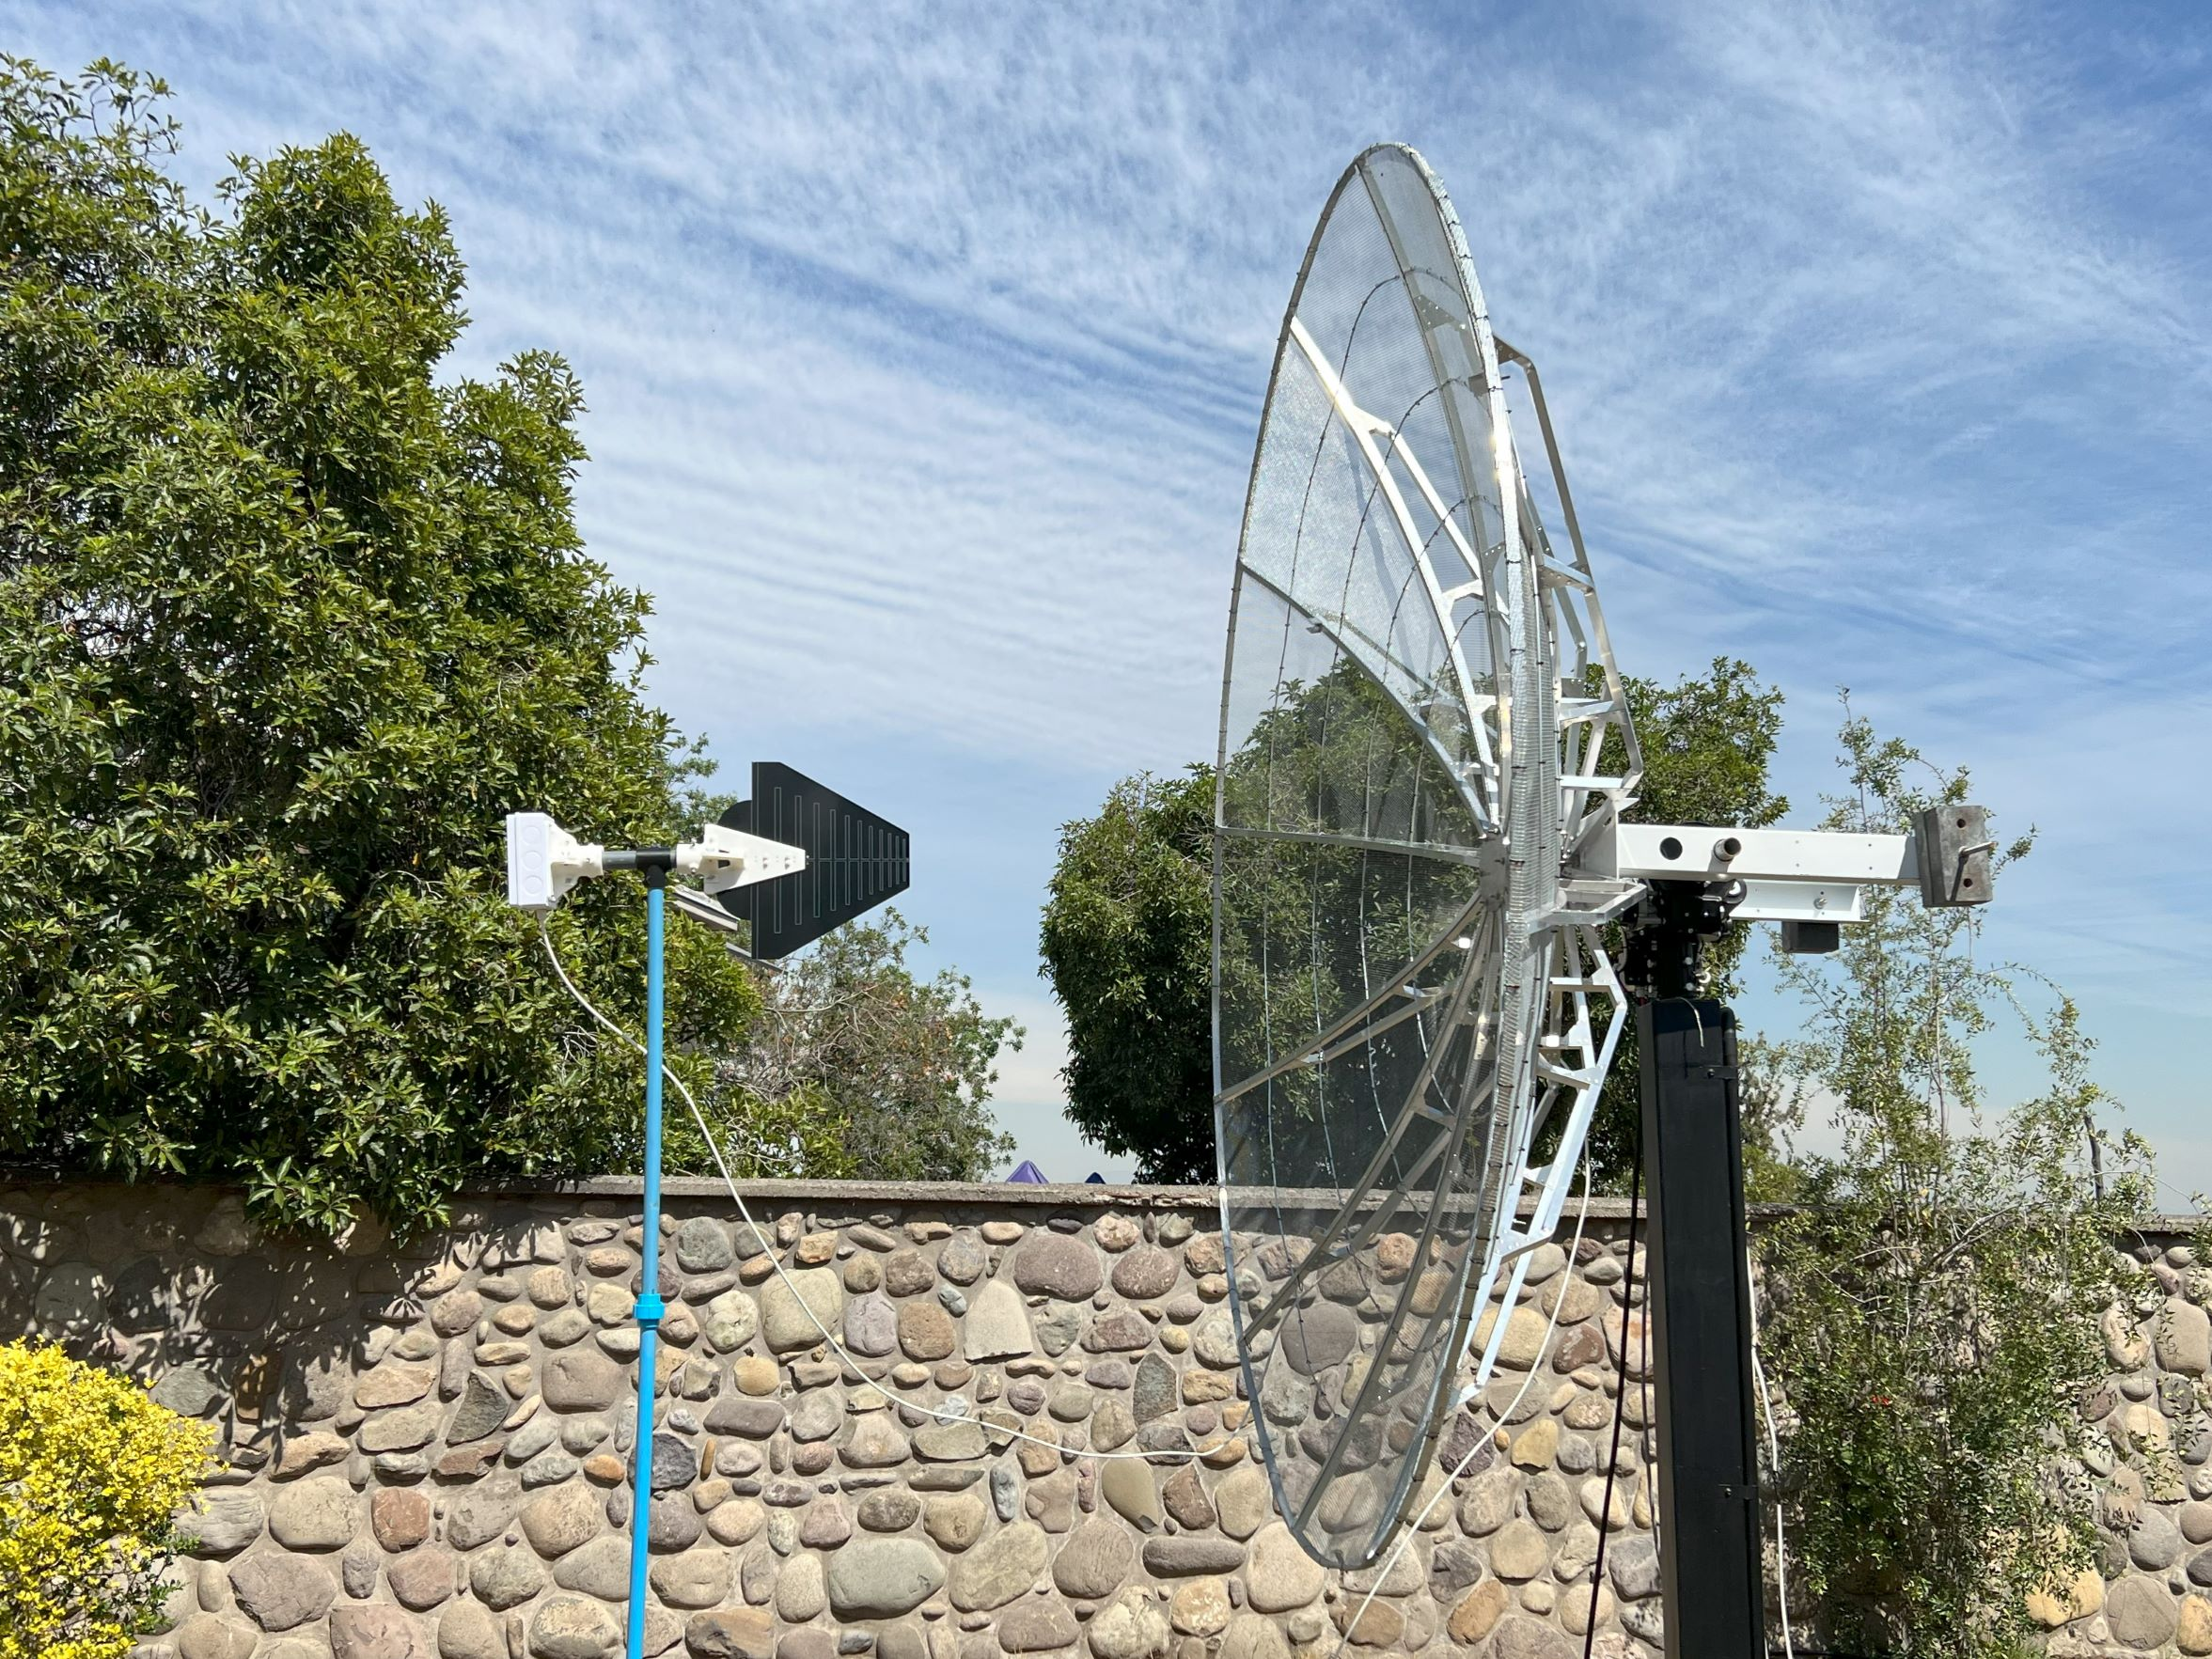
\includegraphics[width=0.7\textwidth]{img/enfoque1}
    \caption{Antena LPDA en trípode auxiliar a 2 metros de altura.}
    \label{fig:antena_lpda}
\end{figure}

Con la antena de la figura \ref{fig:antena_lpda} se procedió a realizar el enfoque del alimentador. La medición consistió en mover el alimentador en el eje Z, es decir, en la dirección de la apertura del reflector. A una distancia de 70 metros desde el reflector se instaló sobre otro trípode un generador de señales portátil con otra LPDA de menor ancho de banda.\\

\begin{figure}[h!]
    \centering
    \begin{subfigure}{0.45\textwidth}
        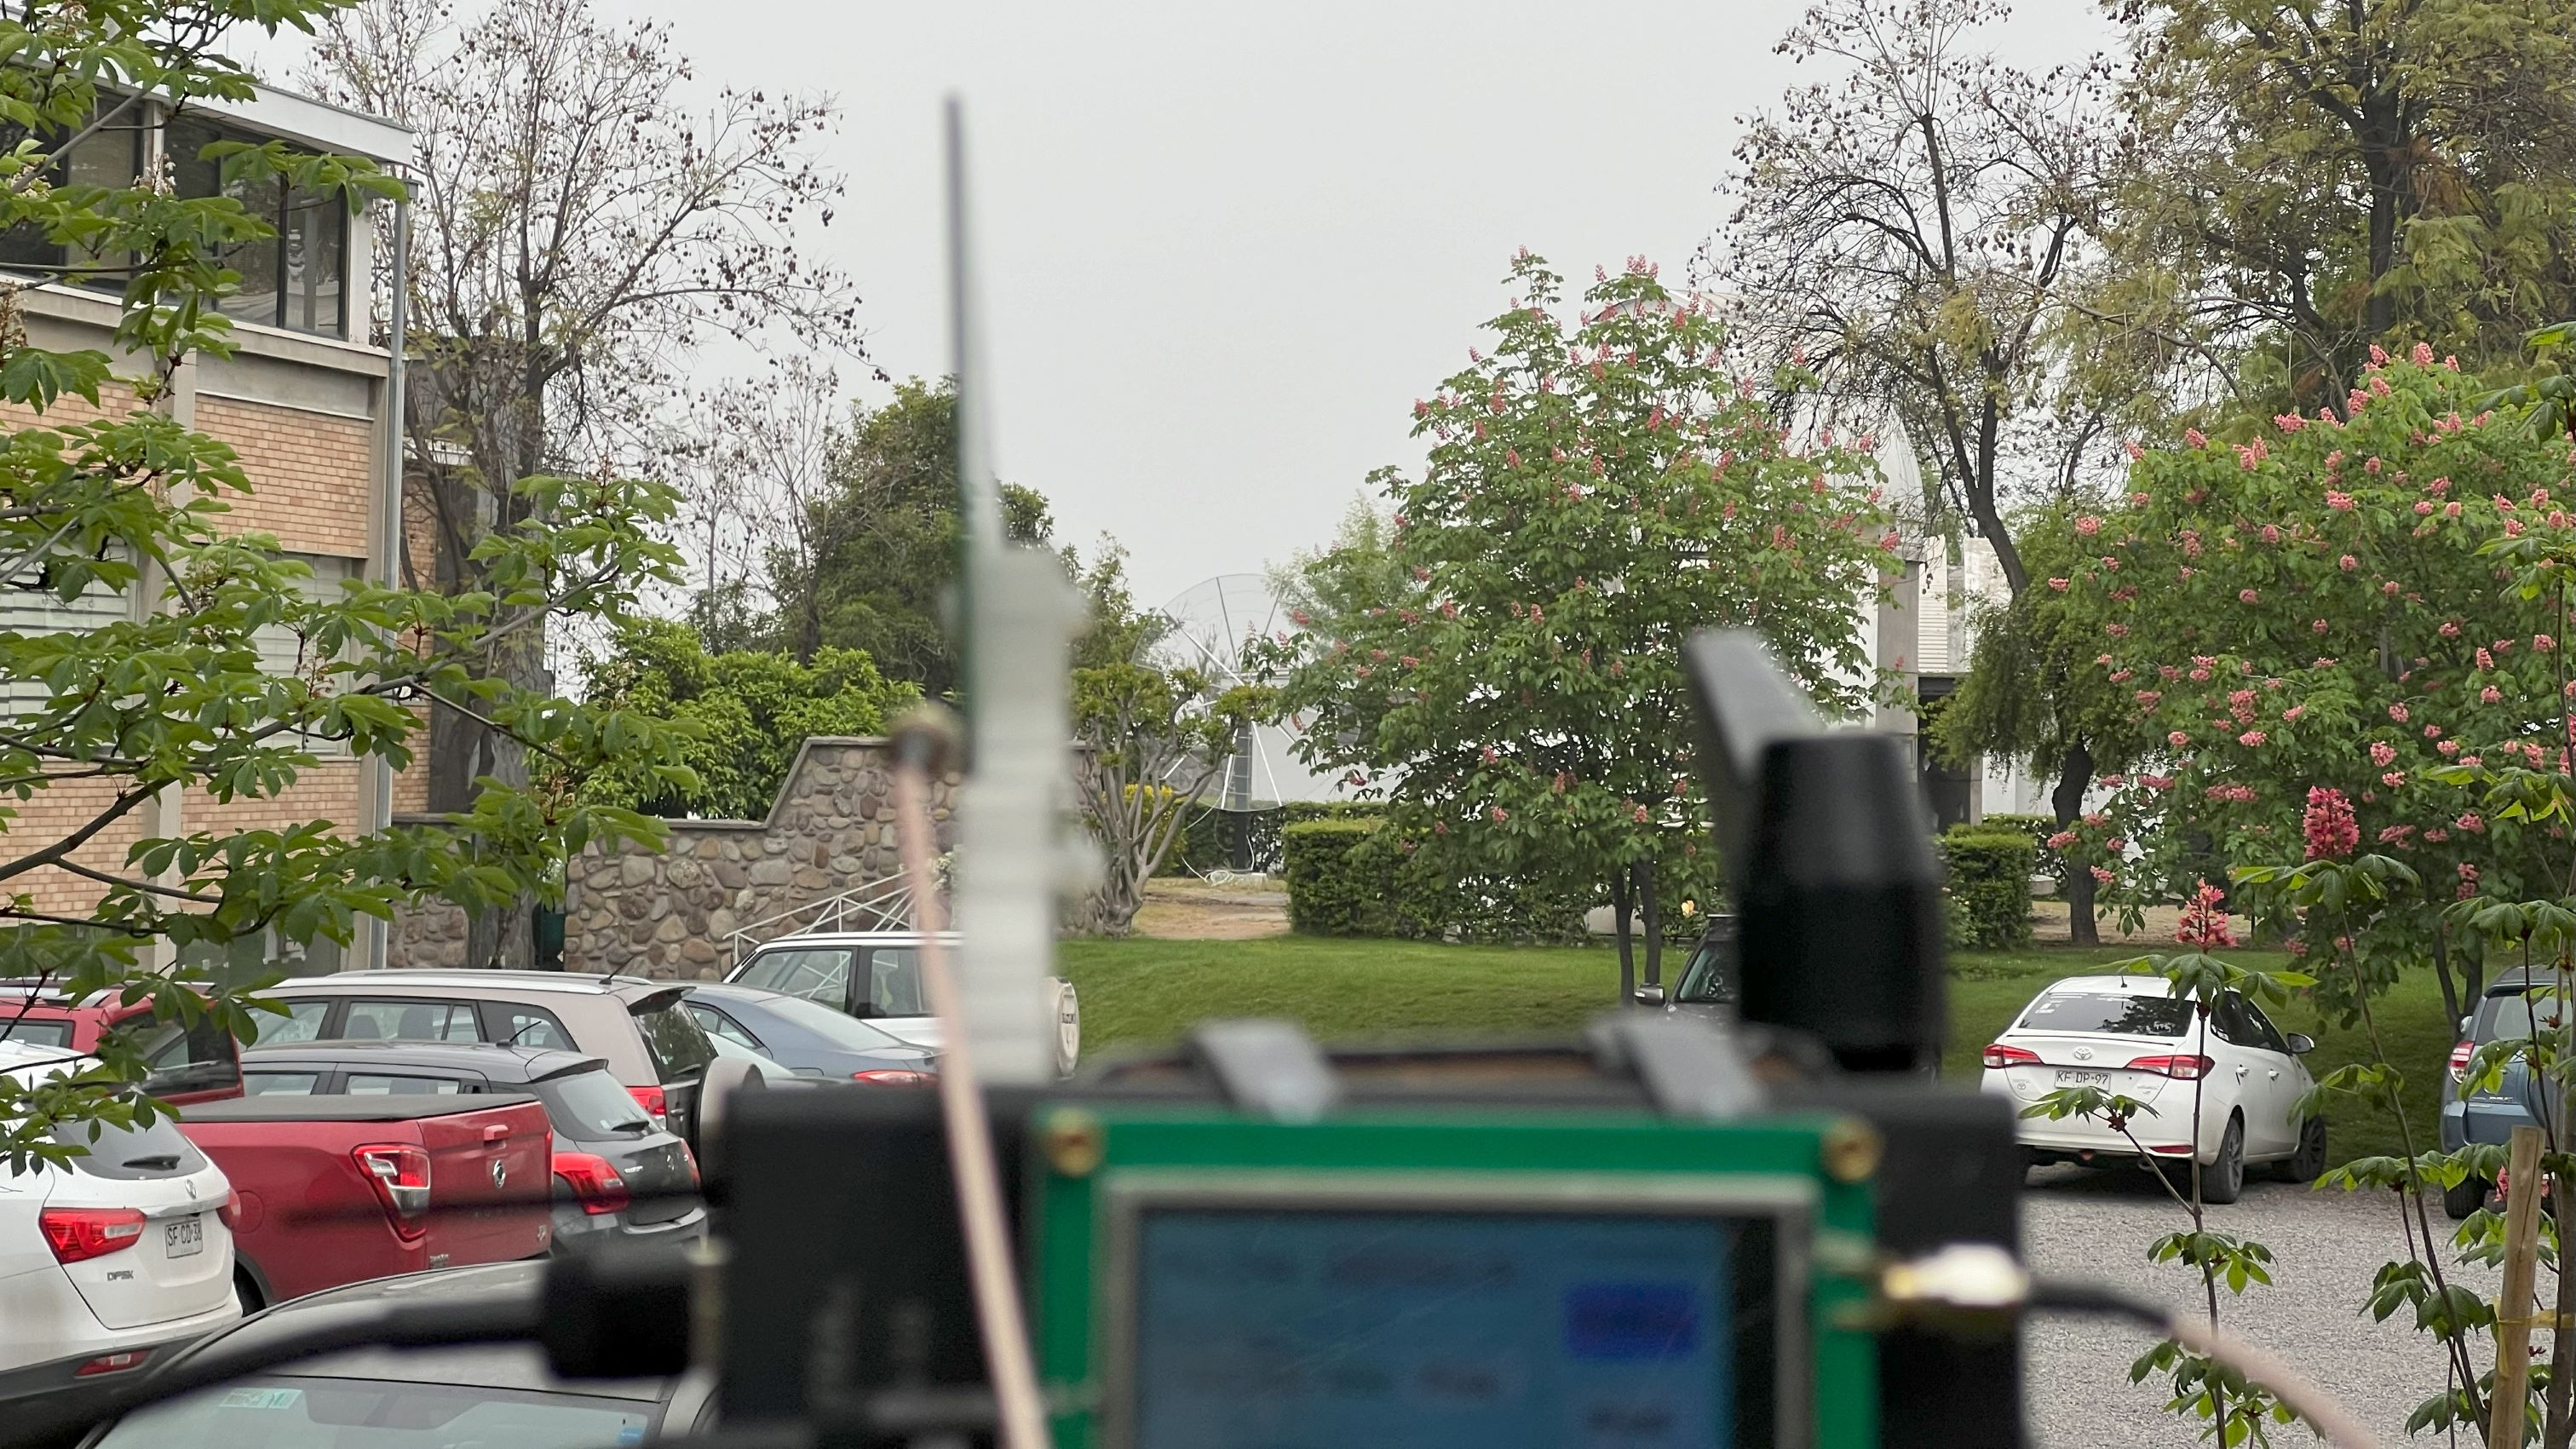
\includegraphics[width=\textwidth]{img/enfoque_cerca}
        \caption{Generador de señales portátil con la antena orientada hacia el reflector a 70 metros.}
        \label{fig:generador}
    \end{subfigure}
    \begin{subfigure}{0.45\textwidth}
        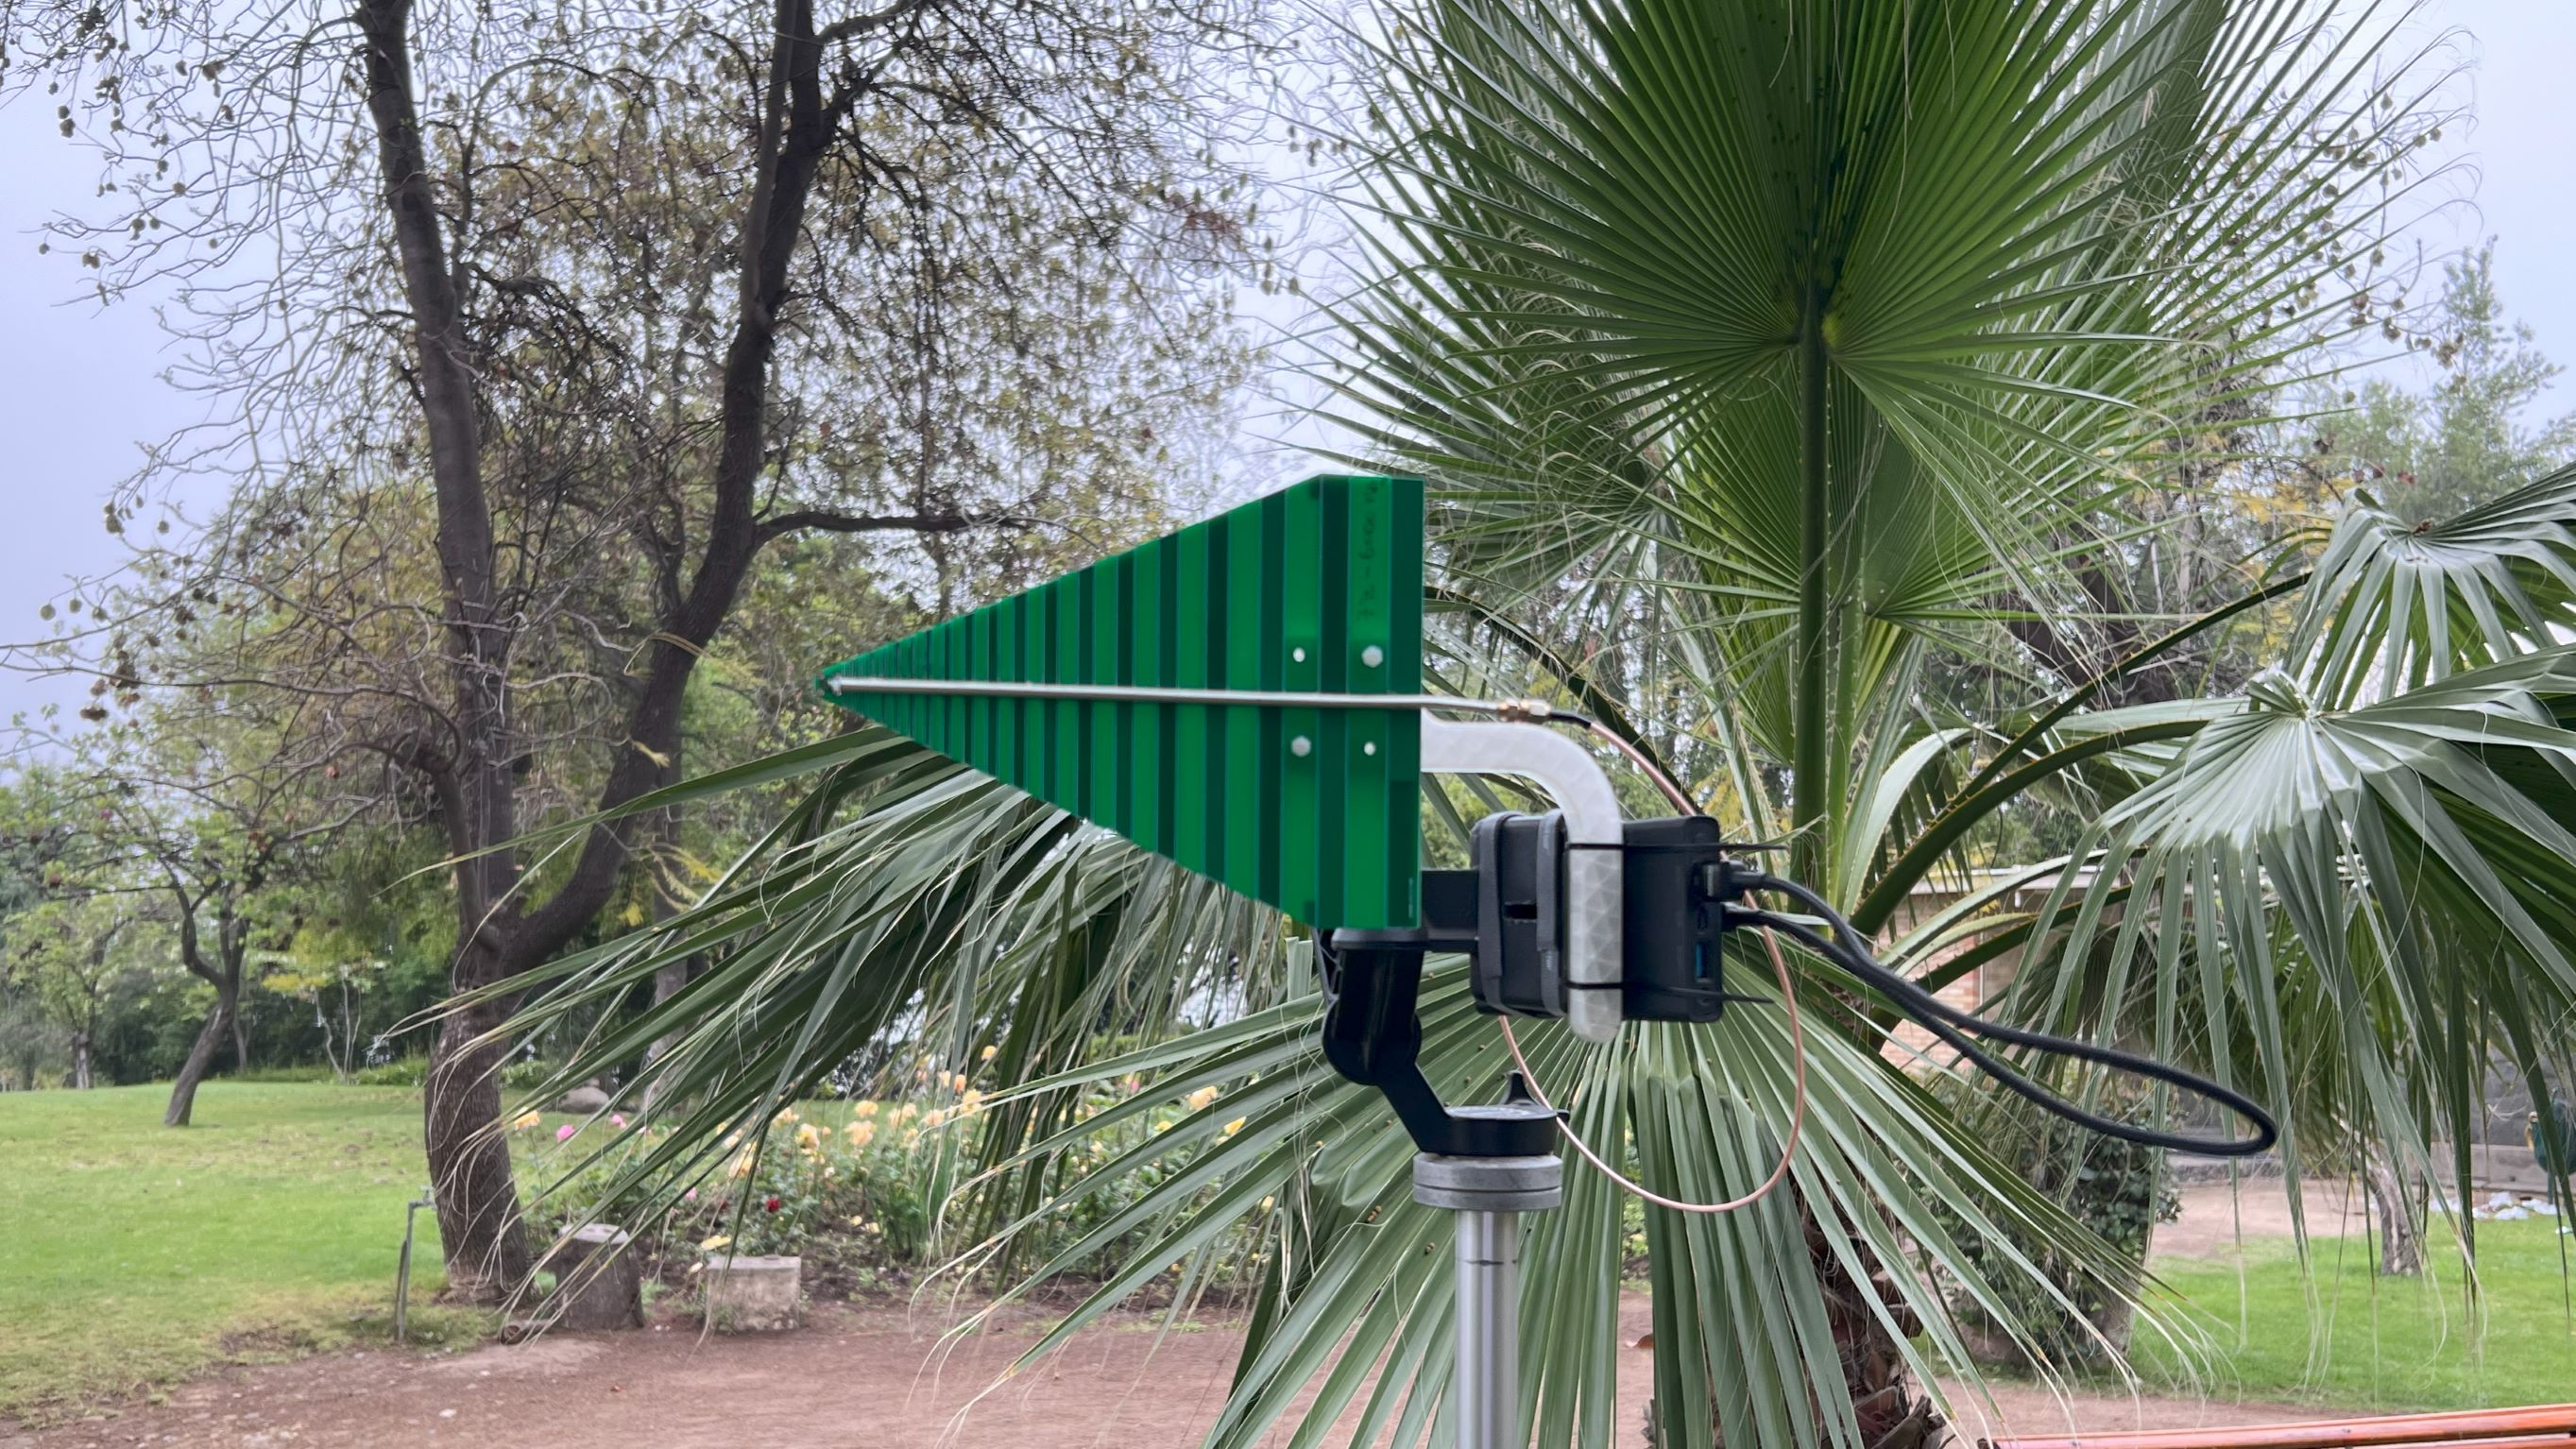
\includegraphics[width=\textwidth]{img/enfoque_cerca1}
        \caption{Antena LPDA de menor ancho de banda instalada con el generador de señales en trípode.}
        \label{fig:antena_lpda}
    \end{subfigure}
\end{figure}

El generador de señales se configuró a una frecuencia de 1000 MHz y se disparó constantemente el tono en dicha frecuencia. Se instaló a una distancia de 70 metros dentro del parque cerro Calán con la consideración de un campo lejano de 60.5 metros a 1000 MHz para el tamaño del reflector, por lo que este generador se encontraba a dicha distancia del reflector.\\

\begin{figure}
    \centering
    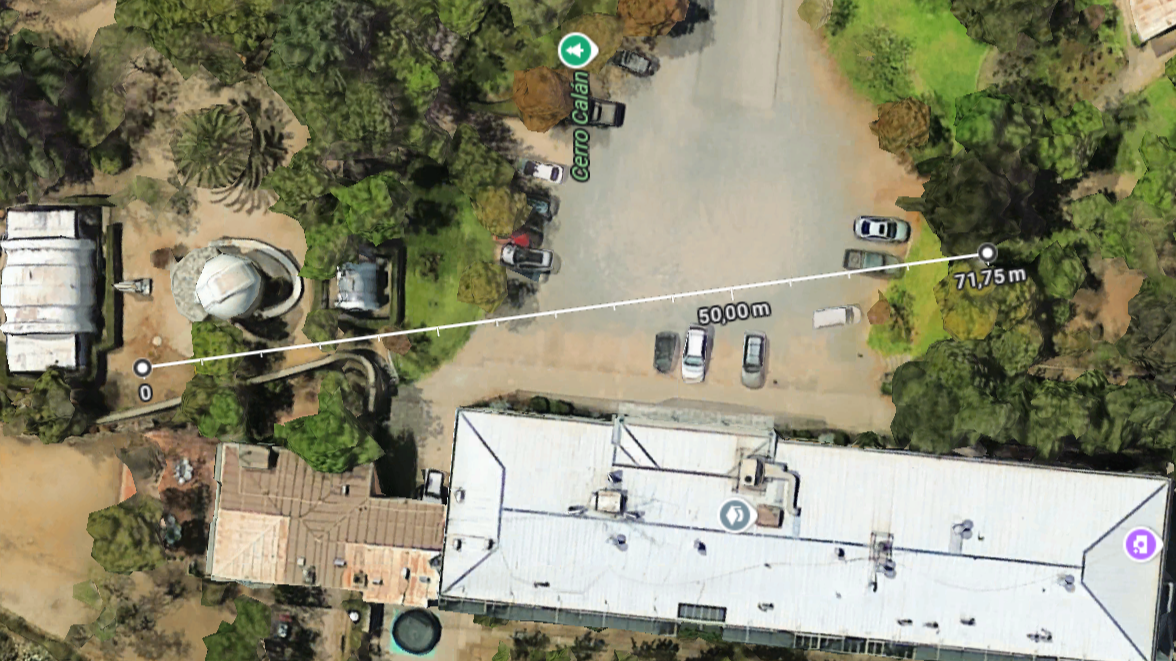
\includegraphics[width=0.7\textwidth]{img/70m_measure}
    \caption{Distancia de 70 metros entre el reflector y el generador de señales con elevaciones similares.}
    \label{fig:70m_measure}
\end{figure} 

En la figura \ref{fig:70m_measure} se muestra la distancia aproximada de 70 metros, tomando 10 metros de distancia adicional para asegurar el campo lejano a dicha frecuencia. Se alineó visualmente la antena del generador con el reflector a la distancia, con una línea de vista que se encontraba parcialmente  obstaculizada por árboles y arbustos.\\

Para efectos de la medición, como se necesitaba encontrar un punto aproximado de enfoque, la exactitud de esta medición no fue crítica. Se procedió a mover el alimentador en el eje Z, es decir en la dirección de la apertura del reflector, hasta encontrar el punto donde la señal del generador era máxima.\\

La potencia recibida por el receptor fue medida con el software de medición utilizando la RTL-SDR guardando los espectros para distancias de 5 cm en 5 cm. Se midió la razón señal a ruido y se obtuvo el punto de máxima potencia recibida en dBFS. Medidas que luego fueron calibradas en dBm por la medición de sensibilidad.\\

\subsection{Alimentador con soportes con la estrella artificial}

Para la medición de enfoque con la estrella artificial se instaló el soporte tetrápodo y se colocó el alimentador en su posición final después de las mediciones anteriores. Se configuró el generador de señales Valon de la estrella artificial a 1428 MHz. Se utilizó esta nueva frecuencia para evitar interferencia de radiofrecuencia en la medición, utilizando el filtro delgado de H1.\\

\begin{figure}
    \centering
    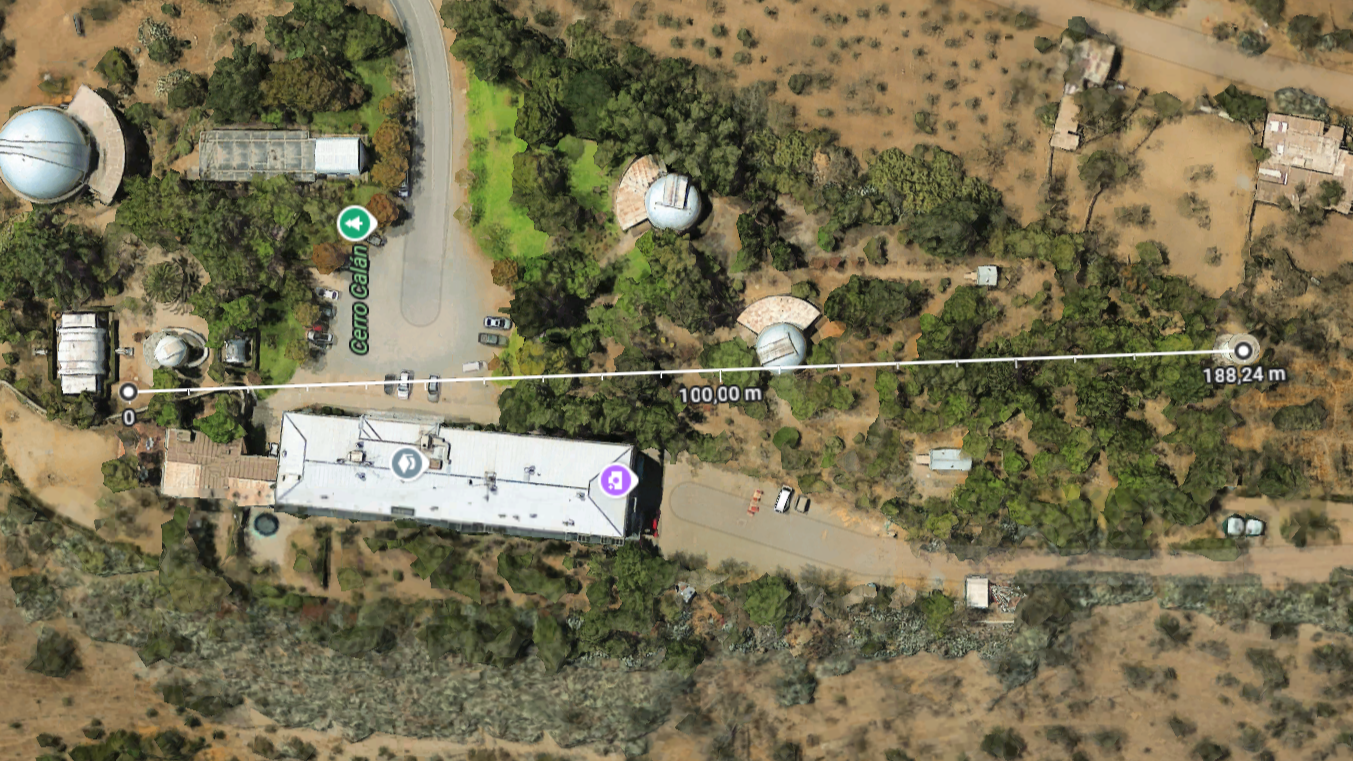
\includegraphics[width=0.8\textwidth]{img/188m_measure}
    \caption{Distancia de 188 metros entre el reflector y la estrella artificial de la copa de agua.}
    \label{fig:enfoque2}
\end{figure}

Para el caso de 1428 MHz, la distancia de campo lejano era de 85 metros y la estrella artificial de la figura \ref{fig:enfoque2} se encontraba a 188 metros, estando perfectamente en el campo lejano del reflector. Además, la alineación con el reflector se realizó con el control automático de la montura alt azimutal y la línea de vista se encontraba completamente libre para la primera zona de Fresnel.\\

\begin{figure}
    \centering
    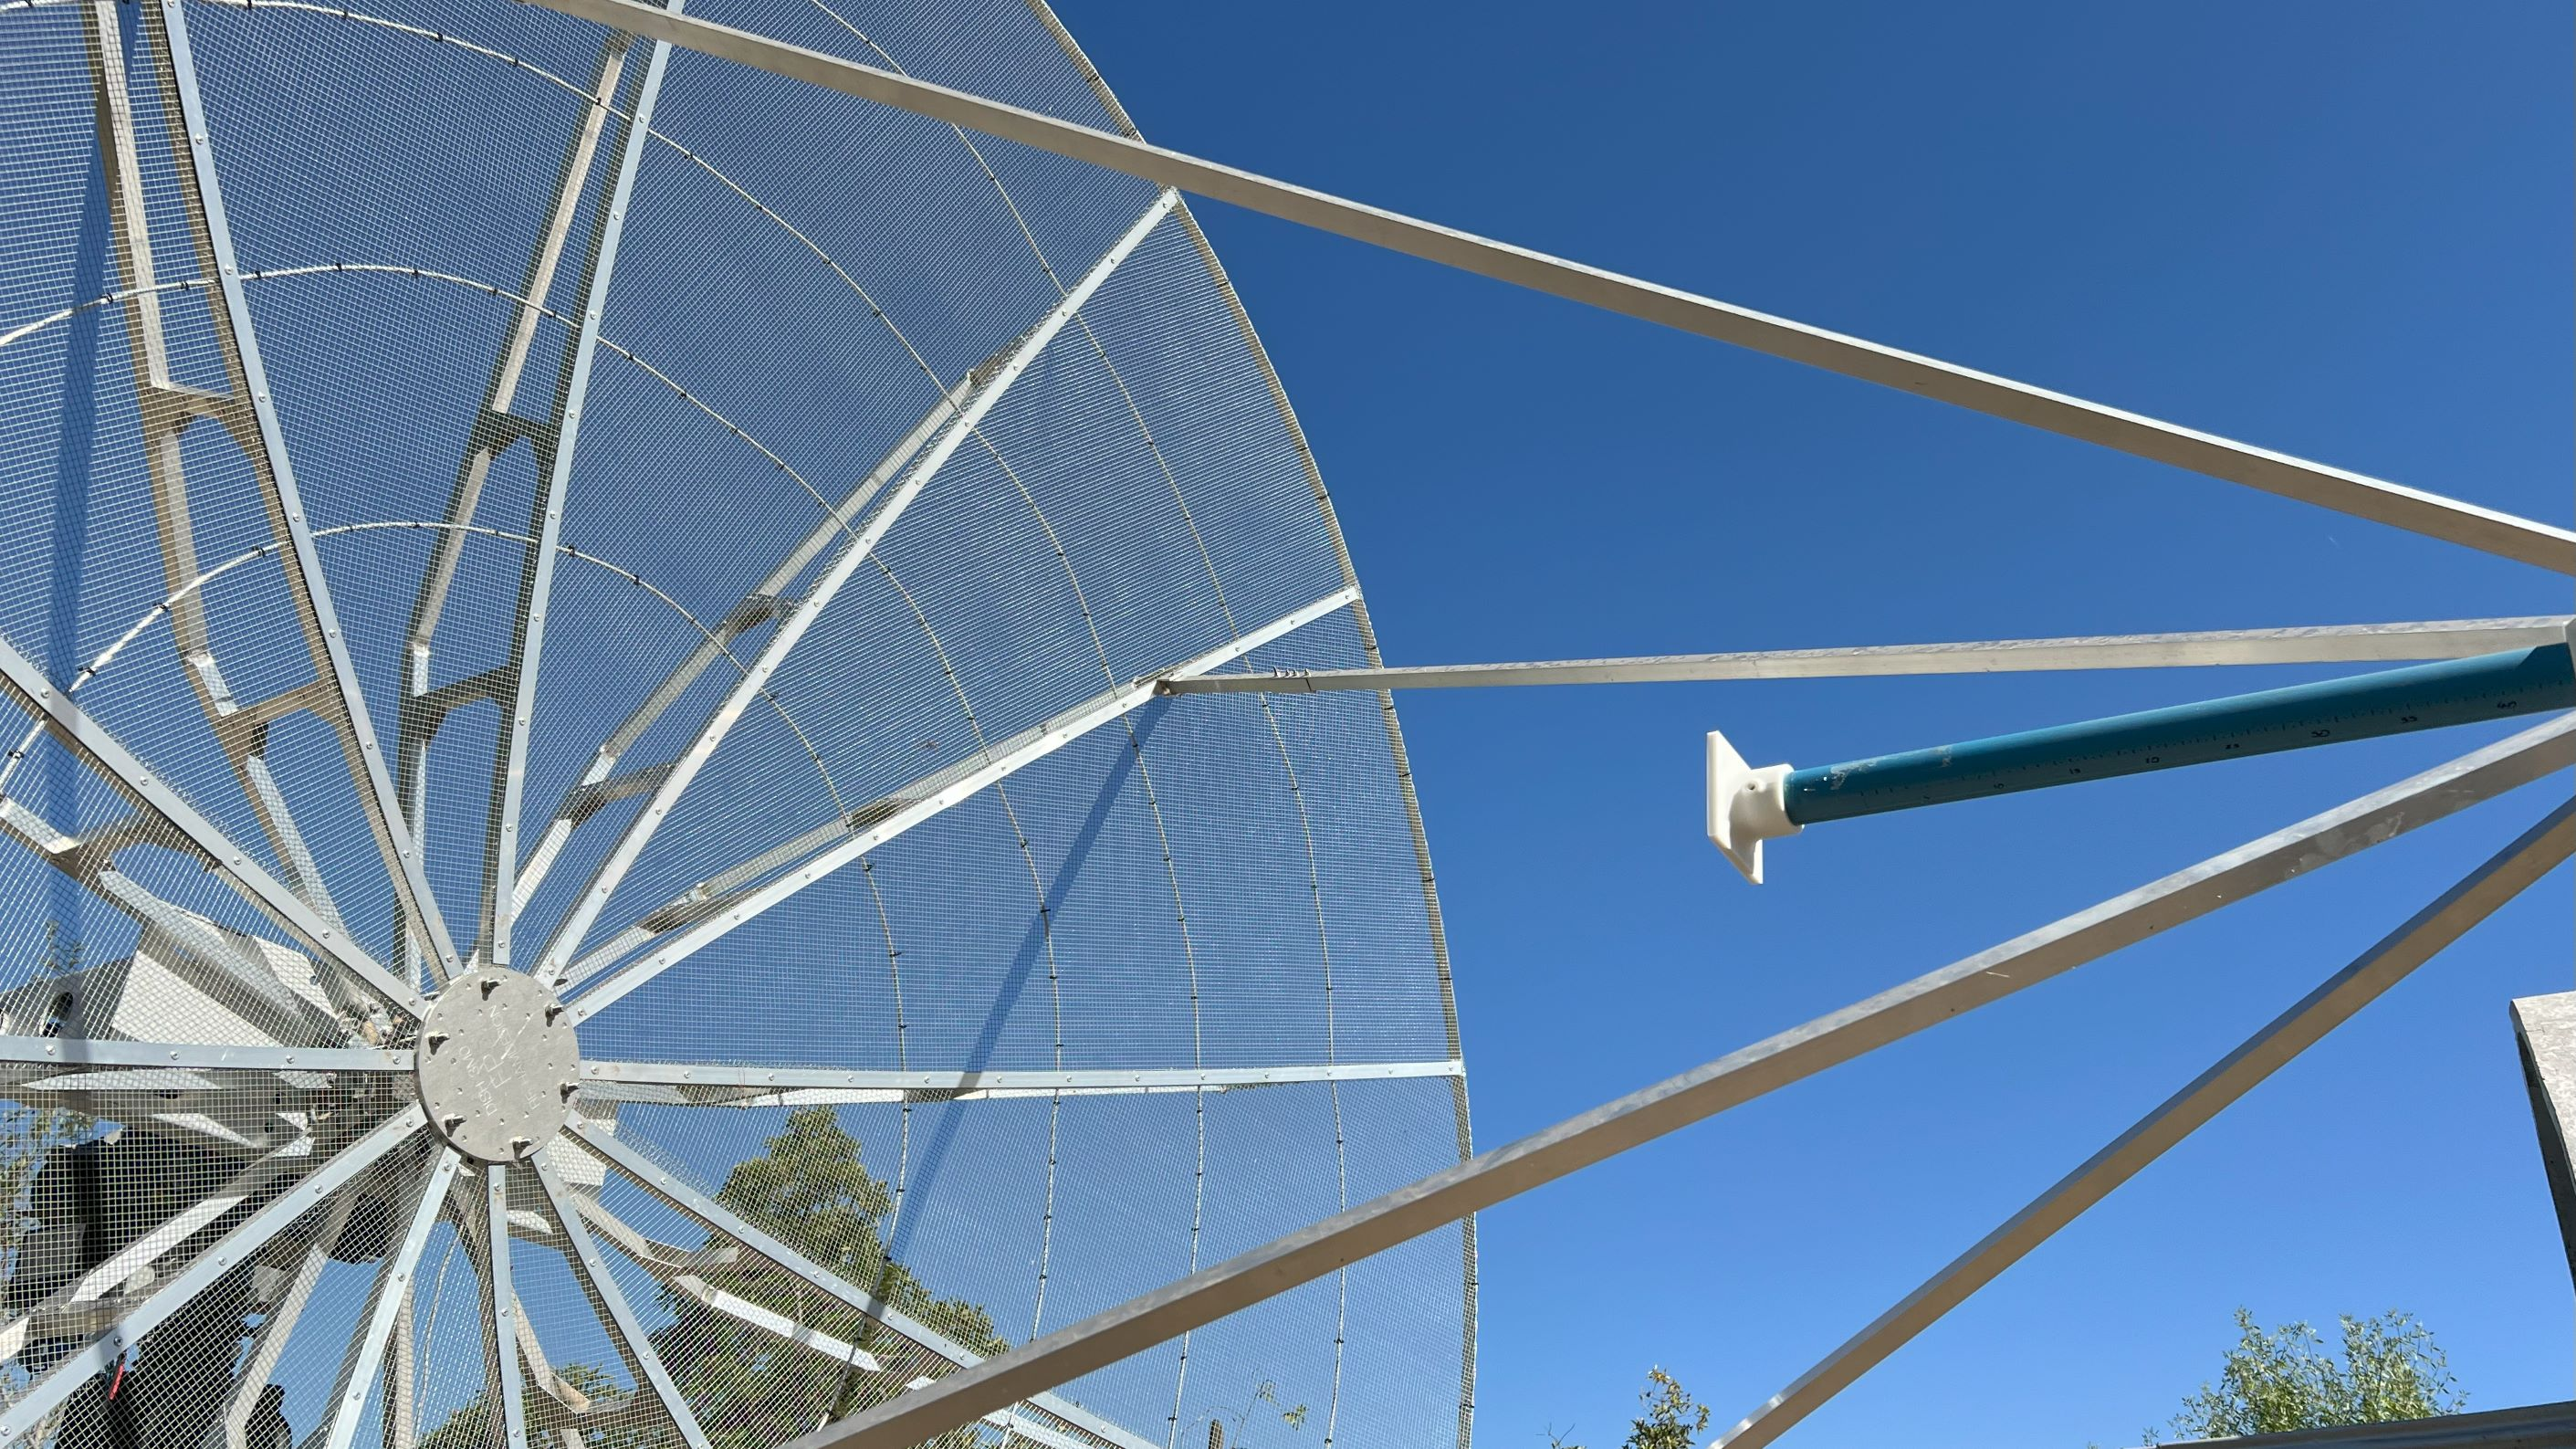
\includegraphics[width=0.7\textwidth]{img/feed_focus}
    \caption{Alimentador dipolo exótico con tetrápodo instalado.}
    \label{fig:enfoque2}
\end{figure}

En la figura \ref{fig:enfoque2} se muestra el alimentador con el tetrápodo instalado y un tubo PVC milimetrado para medir la distancia relativa al reflector, usando de referencia el punto donde los soportes se unen al tubo del alimentador.\\

Para esta medición de enfoque, se movió el alimentador en el eje Z con una resolución de 0.5 cm hasta encontrar el punto de máxima potencia recibida. Se midió la razón señal a ruido y se obtuvo el punto de máxima potencia recibida en dBFS al igual que en la medición anterior.\\

\section{Medición del patrón de radiación}

Se utilizaron 2 plataformas para la medición del patrón de radiación, una con la medida relativa dBFS obtenida de los espectros de la RTL-SDR y otra con la medida absoluta en dBm obtenida con el analizador de espectros Siglent SVA1075x. Para todas las mediciones se utilizó la estrella artificial de la copa de agua.\\

Todas las mediciones de patrón de radiación se realizaron en la cima del cerro Calán, en la plataforma de observación del telescopio CPT. Para cada frecuencia medida, se hicieron los cortes azimutales y de elevación, o la medida del campo H y el campo E. Todos los cortes son de 180 grados para obtener con claridad los lóbulos laterales y con una resolución de 1 punto por grado.\\


\subsection{Medición relativa para banda de H1}

La medición con la RTL-SDR se realizó a 1428 MHz, utilizando el filtro angosto de la misma frecuencia de \textit{RadioastronomySuplies}. El generador Valon, se configuró a 1428 MHz con una potencia inyectada a la estrella artificial de 0.23 dBm.\\

Las pérdidas ohmnicas del cable coaxial RG316 a 1428 MHz son de 10.5 dB por 10 m, como el cable que alimenta la antena de la copa de agua es de 20 metros, se obtuvo una pérdida de 21 dB. La potencia recibida por la antena es de -21 dBm aproximadamente.\\

Con los softwares de medición se obtuvieron los espectros de la señal recibida por la RTL-SDR, se midió la razón señal a ruido y se guardaron 1000 espectros para cada grado de elevación y azimuth. Como la copa de agua se encuentra en altura, se generó un plano semicircular elevado en 7 grados sobre el eje horizontal, donde se corrigieron los valores de elevación por ángulo azimutal con la ecuación de corrección \ref{eq:powerdensity}. Para el segundo corte, se generó un desfase de 7 grados en elevación, y para medir de 0 a -90 grados, se invirtió la posición azimutal en 180 grados para obtener ese cuadrante.\\

\subsection{Medición absoluta para todas las bandas de interés}

\section{Sensibilidad y temperatura de ruido}

La medida de sensibilidad se realizó inyectando un tono para cada frecuencia de interés en la entrada de la cadena de recepción. Se utilizó el generador de señales \textit{Rode \& Schwartz} SMB100A con una potencia de salida de -80 dBm y un coaxial RG316 de 10 metros al receptor instalado en el foco de la antena. Se midieron los espectros generados por la RTL-SDR para determinar la escala dBFS de la radio y calibrar los demás espectros en potencia.\\

Se guardaron los espectros de 300 MHz, 400 MHz y 500 MHz para cubrir la banda de interés del proyecto CHARTS. También se guardaron los espectros de 1000 MHz, 1428 MHz, 1500 MHz y el límite de digitalización de 1700 MHz.\\

\subsection{Medición de la temperatura de ruido}

Para medir la temperatura de ruido y por ende la figura del receptor, se utilizó la fuente de ruido Agilent 346B con una amplificación de 40dB. Para la cadena de amplificación se utilizó el LNA + Filtro H1 SAWbird+ H1 de Nooelec, el cual se conectó a la fuente de ruido y se midió la potencia de ruido en la salida en el analizador de espectro.\\

Para la temperatura de ruido del receptor, se inyectó la señal de ruido en la entrada del receptor y se midió la potencia de ruido con los espectros de la RTL-SDR en la banda de interés.\\

Para obtener la temperatura del sistema completo se realizó una acumulación de espectros del centro de la galaxia a 1420 MHz y a una región del cielo limpia en concentración de hidrógeno neutro. Consultando a los catálogos de radioastronomía se obtuvo la temperatura de la galaxia y de la región del cielo.\\

Con cada una de estas mediciones se realizó el cálculo de temperatura de ruido con el método de Y-factor y se obtuvo la figura de ruido de la cadena de amplificación, del receptor y del sistema.\\


\section{Medición del error de apuntamiento}

\section{Primera luz}

Para la primera luz, se escogió el centro de la galaxia por varias razones. La primera es que se trata de fuente de radio muy fuerte, fácil de detectar y es bastamente estudiada y catalogada. La segunda razón es que, para la época de medición en los meses de noviembre, diciembre y enero, el centro de la galaxia se encuentra bastante cerca del zenith para la latitud de Santiago, lo que facilita la observación.\\

El centro de la galaxia tiene una ascensión recta de 17 h 45 m 40 s y una declinación -29°00'28'', coordenadas que son ingresadas en el software de control de la montura alt azimutal. Se acumularon espectros por periodos de 2 horas durante 3 días, desde las 10 am hasta las 6 pm, para obtener la máxima cantidad de datos posibles. También se descartaron algunas observaciones dónde el sol se encontraba muy cerca del centro de la galaxia, para evitar la saturación del receptor.\\

Para la observación se configuró el telescopio con el receptor de H1 y con la antena dipolo exótico en el foco geométrico del reflector. Se obtuvieron los espectros de la RTL-SDR y se guardaron en el disco duro para su posterior análisis.\\